\documentclass{article}
\usepackage[utf8]{inputenc}
\usepackage{amsmath}
\usepackage{amssymb}
\usepackage{commath}
\usepackage{cancel}
\usepackage{graphicx}
\usepackage{subcaption}
\usepackage{comment}
\usepackage{cases}
\usepackage{listings}
\usepackage{xcolor}
\usepackage{hyperref}
\usepackage[none]{hyphenat} 
\usepackage{listings}
\usepackage{hyperref}
\hypersetup{
    colorlinks=true,
    linkcolor=blue,
    filecolor=magenta,      
    urlcolor=blue,
    pdftitle={Overleaf Example},
    pdfpagemode=FullScreen,
    }

\urlstyle{same}
\definecolor{codegreen}{rgb}{0,0.6,0}
\definecolor{codegray}{rgb}{0.5,0.5,0.5}
\definecolor{codepurple}{rgb}{0.58,0,0.82}
\definecolor{backcolour}{rgb}{0.95,0.95,0.92}

\lstdefinestyle{mystyle}{
    backgroundcolor=\color{backcolour},   
    commentstyle=\color{codegreen},
    keywordstyle=\color{magenta},
    numberstyle=\tiny\color{codegray},
    stringstyle=\color{codepurple},
    basicstyle=\ttfamily\footnotesize,
    breakatwhitespace=false,         
    breaklines=true,                 
    captionpos=b,                    
    keepspaces=true,                 
    numbers=left,                    
    numbersep=5pt,                  
    showspaces=false,                
    showstringspaces=false,
    showtabs=false,                  
    tabsize=2
}

\lstset{style=mystyle}


\title{Linear Regression}
\author{Autor :\\Rodrigo Tesone}
\date{}

\begin{document}

\maketitle

\section{Introducción}
En este texto voy a desarrollar el concepto de regresión lineal de la manera más precisa y menos técnica posible, es decir, que se entienda el concepto y como aplicarlo sin entrar en las complejidades de las demostraciones matemáticas.\\
Los conceptos matemáticos necesarios para entender este tema se explicaran dentro de este mismo texto pero si se van a necesitar los conocimientos de Python necesarios para hacer las graficas y las regresiones lineales (los códigos están comentados pero no explicados desde 0).\\
Los datos que usaremos en el texto fueron extraidos \href{https://www.kaggle.com/c/house-prices-advanced-regression-techniques/data?select=test.csv}{aquí}.\\
Este texto fue creado con fines educativos. Las comparaciones o aplicaciones mostradas aquí pueden no ser totalmente fidedignas a sus aplicaciones en el mundo investigativo, laboral o académico.

\section{Primera aproximación a la idea}
Cuando se escribe al respecto a este tema muchas veces (no siempre) se busca aplicar el concepto ya definido a casos concretos. Acá
vamos a ir abordando el concepto como si se nos ocurriera a nosotros y luego usaremos Python para complementar nuestro aprendizaje.\newline
 Un problema muy típico con el que se ejemplifica la regresión lineal es el problema del precio de una casa.  El problema es el siguiente:\\\\
\textbf{¿Como podemos predecir el precio de una casa? ¿Basándonos en que factor cambia el precio?} \\\\
Hay varias respuestas a estas preguntas. Uno podría pensar que está relacionado con la cantidad de pies cuadrados de la propiedad, la cantidad de habitaciones, el año en que fue construida, la zona en la que esta construida y un largo etc.\\
Solo para simplificar vamos a ver la relación Área-Precio. Es decir, como aumenta o disminuye el precio de una viviendo a medida que aumenta o disminuye el área de la propiedad.\\
Los puntos que vamos a dibujar en los siguientes gráficos son datos reales extraídos del archivo 
``train.csv”, es decir, son datos ya medidos:
% Unico punto
\begin{figure}[h]
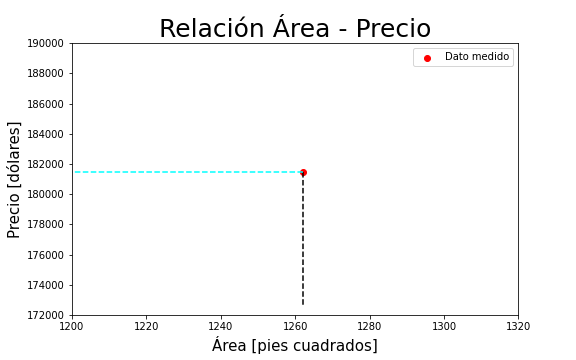
\includegraphics[scale=0.5]{Imagenes/unico_punto.png}
\centering
\end{figure}
\newpage
¿Se entiende este dibujo (que a partir de ahora lo llamaremos grafico)? Dado un área (el eje horizontal) esa área tiene asignada un precio (eje vertical).\\
¿Que pasa si aumento el área? ¿Aumenta el precio? Veamos
% 2 Puntos
\begin{figure}[h]
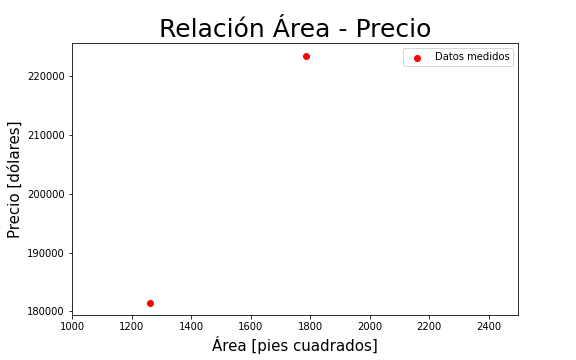
\includegraphics[scale=0.5]{Imagenes/2_puntos.png}
\centering
\end{figure}
\newpage
Como vemos, al movernos a la derecha (osea, aumentar el área de la propiedad) también aumento (se movió más arriba) el precio de la casa.\\
Hasta ahora nada del otro mundo, bastante intuitiva la conclusión.\\
Pero ahora imaginemos que quiero saber el precio de una casa cuya área este entre estos 2 puntos (por ejemplo 1500 pies cuadrados). Podemos imaginarnos que va a aumentar el precio respecto al primer punto y bajar el precio respecto al segundo punto ¿Pero cuanto?\\
Para responder esta pregunta podemos ponernos imaginativos y unir los 2 puntos una linea recta así:
% Recta
\begin{figure}[h!]
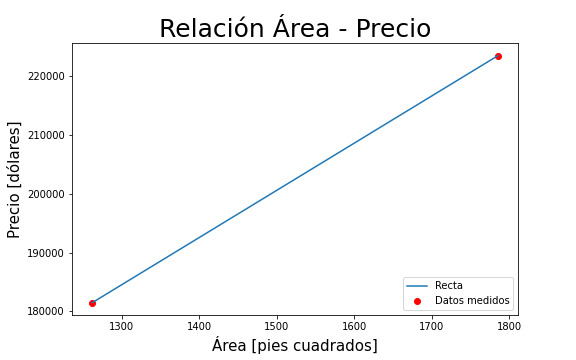
\includegraphics[scale=0.5]{Imagenes/recta.png}
\centering
\end{figure}
\\
Ahora con esta recta podemos (por ejemplo) tratar de adivinar que precio tendrá una casa de 1500 pies cuadrados.\\
¿Como? Miremos
\begin{figure}[h!]
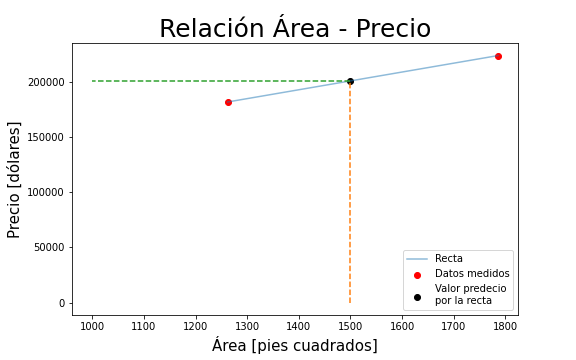
\includegraphics[scale=0.5]{Imagenes/prediccion_valor_1500.png}
\centering
\end{figure}
\newline
Ahí vemos como nos paramos en los 1500 pies cuadrados y luego buscamos cuando se ``choca” con la recta, una vez que nos chocamos con la recta vemos que precio tiene (en este caso 200000 dólares).\\
Bien, problema resuelto. Ahora somos unos expertos en precios de casas ¿No?\\
¿Y si ponemos 3 puntos?\\
% 3 Puntos
\begin{figure}[h]
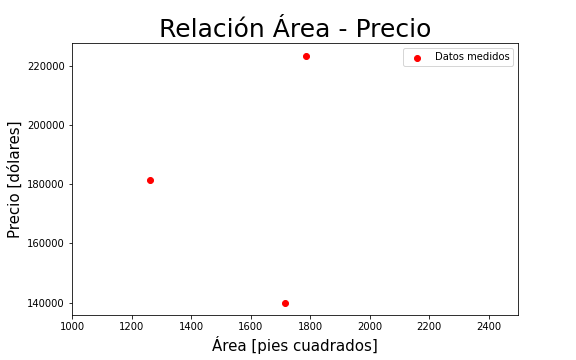
\includegraphics[scale=0.6]{Imagenes/3_puntos.png}
\centering
\end{figure}
\newpage
¿Y si ponemos 10 puntos?\\
% 10 Puntos
\begin{figure}[h!]
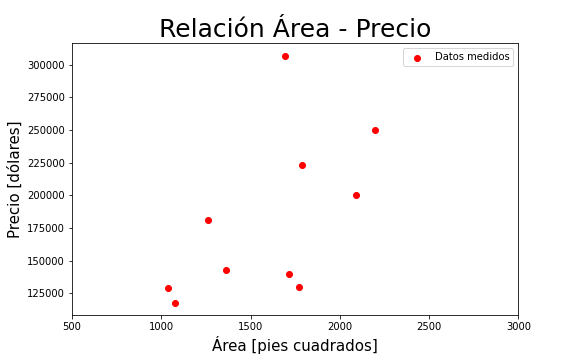
\includegraphics[scale=0.5]{Imagenes/10_puntos.png}
\centering
\end{figure}
\\
¿Y si ponemos todos los puntos?\\
% Todos los puntos
\begin{figure}[h]
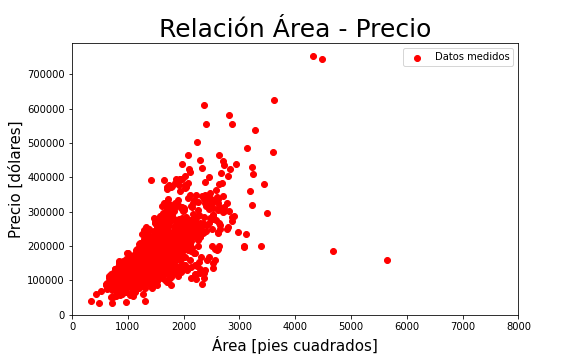
\includegraphics[scale=0.5]{Imagenes/todos_los_puntos.png}
\centering
\end{figure}
\newpage
Ahora se nos presenta un gran problema, no podemos observar con claridad el precio asociado a una determinada área (en esa nube de puntos es casi imposible ver que precio tiene una vivienda de 2000 pies cuadrados por ejemplo).\\
Además podemos observar que es imposible que una recta que pase por todos los puntos al mismo tiempo asique cambiemos la estrategia, hagamos que la recta se aleje lo menos posible de los puntos, es decir, que el \textbf{error} (la distancia) entre la recta y los puntos sea \textbf{mínima}.\\
En otras palabras, vamos a tratar de obtener una recta que se aleje AL MISMO TIEMPO lo menos posible de todos los puntos y por ende que la distancia entre la recta y los puntos sea la menor posible.\\
¿Como podemos hacer eso?\\
Es complejo explicar como hacer eso sin meterse en conceptos matemáticos avanzados (por ejemplo, derivadas de funciones de una sola variable). Lo que si podemos hacer es usar Python para ayudarnos a simplificar esta tarea.\\
 Pero antes de seguir con esto vamos a tratar de explicar matemáticamente el concepto de grafico y recta.

\section{Hablemos de matemáticas}
Imaginemos tenemos una tabla así:
\begin{center}
 \begin{tabular}{|c | c|} 
 \hline
 x & y \\
 \hline
 0 & 0 \\ 
 \hline
 1 & 2 \\
 \hline
 2 & 4 \\
 \hline
 3 & 6 \\
 \hline
 4 & 8 \\ [1ex] 
 \hline
\end{tabular}
\end{center}
Ahora vamos ubicando estos puntos, es decir, me paro en la $x$ y luego subo hasta el valor $y$.\\
Si grafico esos puntos en un plano cartesiano (el plano x-y) tenemos:\\
% Plano x-y
\begin{figure}[h!]
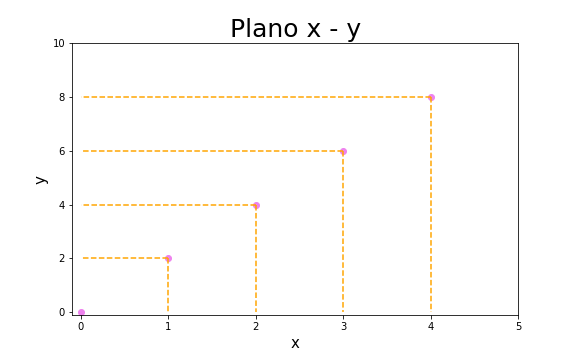
\includegraphics[scale=0.5]{Imagenes/plano_x_y.png}
\centering
\end{figure}
\newpage
Si hacemos como cuando eramos niños y unimos los puntos podemos hacer lo siguiente:\\
% Recta de Prueba
\begin{figure}[h!]
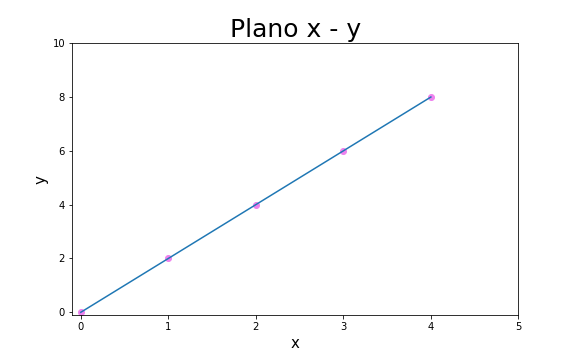
\includegraphics[scale=0.5]{Imagenes/recta_de_prueba.png}
\centering
\end{figure}
\newline
¿Entonces cada vez que quiera hacer una recta tengo que escribir una tabla de números? Pues no, los matemáticos que son gente con bastante tiempo libre e imaginación se les ocurrió otra manera (más simple) de hacer esto.\\
Miremos este ejemplo\\
\begin{equation*}
    y= 2 \cdot x
\end{equation*}
Ahí lo que vemos es una ecuación con 2 variables. Una independiente (x) y una dependiente (y).\\
¿Como funciona esto? Es bastante sencillo, vas reemplazando la x por un número, se multiplica por 2 y se obtiene el valor de y.\\
 Por ejemplo si reemplazo $x=0$:
\begin{equation*}
    \begin{split}
        y &=2\cdot 0\\
        y &=0
    \end{split}
\end{equation*}
Si reemplazo $x=1$:
\begin{equation*}
    \begin{split}
        y &=2\cdot 1\\
        y &=2
    \end{split}
\end{equation*}
Y así podemos ir reemplazando con otros valores y podemos obtener la tabla que vimos al principio.\\
Ahora que ya entendimos un poco como ``funciona” una recta analicemos un poco más.\\
¿Que pasa si aumento o disminuyo el numero que multiplica la x?\\
% Distintas pendientes
\begin{figure}[h!]
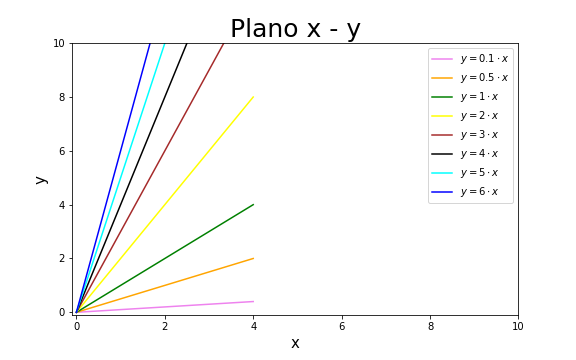
\includegraphics[scale=0.5]{Imagenes/distintas_pendientes.png}
\centering
\end{figure}
\newpage
Se puede observar que entre más grande es el número que multiplica a la $x$
 más pronunciada es la pendiente. Imaginate que tenes que subir una rampa ¿Cual preferirías subir? ¿La rosa o la azul? Te dejo la tarea de pensar que pasa si el número que lo multiplica es negativo.\\
 Ahora en vez de multiplicarles distintos números vamos a sumar o restarle distintos números y veremos que pasa con la grafica.\\
% Distintas ordenadas al origen
\begin{figure}[h!]
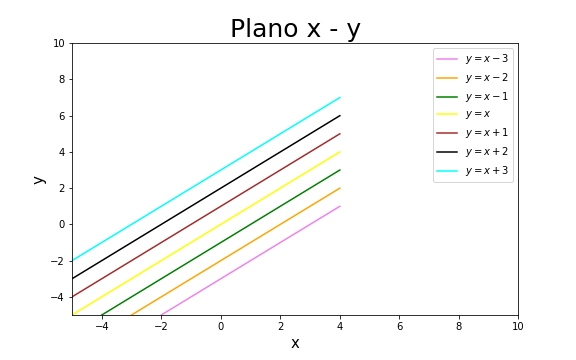
\includegraphics[scale=0.5]{Imagenes/distinta_ordenada_al_origen.png}
\centering
\end{figure}
\newline
Como vemos, lo que cambia acá es que la recta sigue estando igual de inclinada (tiene la misma pendiente) pero la recta esta más arriba o más abajo (se traslada) depende si se suma o resta el número a la $x$.\\
\section{Volvamos al problema}
Una recta esta hecha con esta ecuación:
\begin{equation*}
    \textcolor{blue}{y} = \textcolor{red}{m}\cdot \textcolor{green}{x} +\textcolor{orange}{h}
\end{equation*}
Donde:
\begin{align*}
    \textcolor{blue}{y} &= \text{ variable dependiente}\\
    \textcolor{green}{x} &= \text{ variable indepediente}\\
    \textcolor{red}{m} &= \text{ pendiente}\\
    \textcolor{orange}{h} &= \text{ ordenada al origen}
\end{align*}
En el ejemplo que estábamos viendo la variable independiente seria los pies cuadrados y la dependiente seria el precio de la vivienda.\\
Recordemos que nuestro objetivo era construir una recta para hacer más fácil obtener el precio de una vivienda dado el área de la propiedad.\\
El problema acá es que no sabemos que valor es $m$ y que valor es $h$ para la recta que queremos obtener.\\
Con unas líneas en Python obtenemos los valores:
% Aca va el codigo
\begin{lstlisting}[language=Python]
# Importo los paquetes necesarios para la Regresion lineal

from sklearn.model_selection import train_test_split
from sklearn.linear_model import LinearRegression

# Defino como dataframe el archivo de entrenamiento

df = pd.read_csv("train.csv")

# Defino los valores de la variable independiente y la dependiente

x = df["GrLivArea"].values.reshape(-1,1)
y = df["SalePrice"].values.reshape(-1,1)

# Entrenamos el set de  datos
# El  modulo train_test_split recibe el set de datos, los divide en
# 2 partes (en este caso es un 80 % de entrenamiento y
# 20 % de testeo) y asi se tiene separados los datos para
# entrenar el modelo y testearlo

X_train, X_test, y_train, y_test = train_test_split(x, y,
    test_size =0.2,random_state=0)

# Inicializo la clase LinearRegression

modelo = LinearRegression()

# En esta linea se entrena el modelo, es decir, le damos los  datos
# al modelo y asi obtener los valores de la recta

modelo.fit(X_train , y_train)

# Obtenemos la pendiente redondeada a 2 decimales:

pendiente=round(modelo.coef_[0][0] ,2)
print(f"La pendiente (m) de la recta es: {pendiente}\n")

# Obtenemos  la  ordenada  al  origen  redondeada a 2 decimales:

ordenada_al_origen=round(modelo.intercept_ [0],2)
print(f"La ordenada al origen (h) de la recta es: {ordenada_al_origen}\n")

# Obtenemos la eficiencia del modelo

eficiencia_modelo=round(modelo.score(X_test,y_test),2)*100
print(f"El modelo tiene una eficiencia del {eficiencia_modelo} %")
\end{lstlisting}
$\therefore$
\begin{equation*}
    y=110.26\cdot x+13330.29
\end{equation*}
Es la recta que tanto buscamos.\\
Y si la graficamos tenemos:
% Recta Final
\begin{figure}[h!]
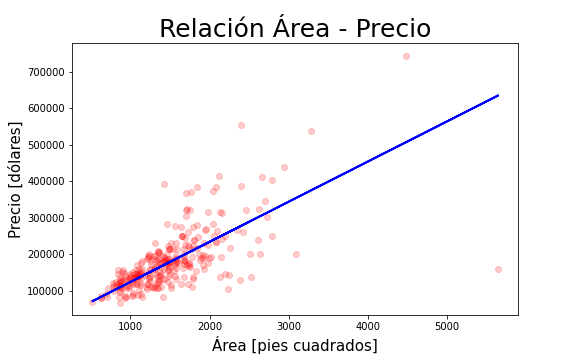
\includegraphics[scale=0.5]{Imagenes/recta_final.png}
\centering
\end{figure}
\newpage
\section{Y todo esto ¿Para que?}
Todo este esfuerzo puede parecer poco interesante, pero dejame convencerte de que vale la pena.\\
Imaginemos que quisieras tasar una propiedad con determinados pies cuadrados ¿Como lo harías?\\
Es una buena idea basarte en los datos que ya tenes para tener una noción de los precios de mercado. Con esa lógica, tendrías que ver la nube de puntos difusa que vimos antes y luego encontrar el valor que estábamos buscando. ¿Que tan practico parece eso? Es como buscar una aguja en un pajar.\\
Otro problema es que los datos son finitos, lo que significa que no puedo medir el precio para todas las áreas posibles (por ejemplo, para 1685 pies cuadrados no hay un precio asociado) ¿Como le ponemos precio? No basta solo ponerle un precio ``a ojo”, hay que basarse en algún tipo de análisis al respecto.\\
Por último (y quizá más importante) observemos que pasando los 3000 pies cuadrados hay muy pocos datos, con esta recta se puede \textbf{predecir} valores que no conocemos y eso es un poder gigante.\\
Pensemos que estamos en una inmobiliaria y tenemos que tasar una casa de 4000 pies cuadrados. Como vemos no hay una medición directa para tener de referencia y ya dijimos que eso de
``mirar a ojo” no es la mejor solución.\\
Es realmente un problema complejo, imaginemos que pongo un precio desorbitante que no se equipara a los precios con pies cuadrados similares. En ese caso es probable que tarde más tiempo en encontrar un vendedor que quiera adquirirla casa (si es que la adquiera) y el tiempo es un factor importante al momento de vender un producto.\\
Entonces la idea es encontrar el mejor precio posible (lo suficientemente accesible para no tener a la casa sin vender por mucho tiempo pero tampoco tan barato para perder dinero en la venta).\\
Si valuamos $x=4000 \text{ pies cuadrados}$ en la recta tenemos:
\begin{equation*}
    \begin{split}
        y&=110.26\cdot 4000+13330.29\\
        y&=454370.29 \text{ dolares}
    \end{split}
\end{equation*}
Y ese es solo un ejemplo de como usar la recta para poder predecir un resultado, dar respuestas a preguntas concretas y resolver un problema.

\section{Discrepancia entre valor real y valor del modelo}
Veamos esta imagen:
% Error
\begin{figure}[h!]
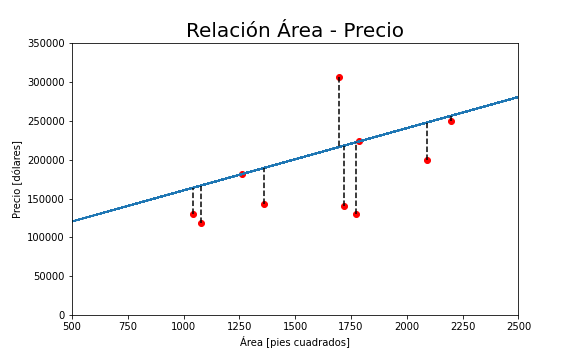
\includegraphics[scale=0.5]{Imagenes/error.png}
\centering
\end{figure}
\newpage
¿No les da dudas que se alejen tanto los puntos reales de la recta? ¿Y si cuando usamos la recta para predecir el numero esta muy lejos del valor medido?\\
Recordemos que la recta es un \textbf{modelo}, una aproximación de los datos, no necesariamente tiene que dar los valores exactos de cada medición.\\
Un modelo (si es bueno) se encarga de que haya la menor de diferencia entre los valores reales y nuestro modelo así en vez de usar una nube de puntos horrible usamos nuestro lindo (a veces) modelo.\\
Sacrificamos un poco de exactitud en pos de ganar mucha simplicidad para la predicción y la lectura de datos.\\
No es una practica nada fuera de lo normal, en muchos ámbitos de la ciencia y la tecnología se utilizan modelos, se descartan valores, se aproximan otros para lograr predicciones del fenómeno que estamos estudiando.

\section{Problemas mas complejos}
Bien, hasta ahora entendimos como poder aproximar el precio de una casa en función de su área.\\
Pero como imaginamos el precio de una casa tiene más factores que su área. Veamos otro factor, los metros cuadrados de la cochera.¿Como hacemos para tener en cuenta este factor? Pues con matemáticas, por supuesto.\\
Primero hay que ver como dibujar esto.\\
La primera medición tiene estos 3 valores:
\begin{equation*}
    \begin{split}
        x&=2376 \text{ pies cuadrados}\\
        y&=853 \text{ pies cuadrados}\\
        z&=325300 \text{ dólares}
    \end{split}
\end{equation*}
Ubiquemos este punto en un grafico x-y-z (3 dimensiones).\\
Lo que hacemos basicamente es primero ubicar en un grafico 2D el valor de x e y asi.\\
Primero nos ubicamos en el eje x:\\
\begin{figure}[h!]
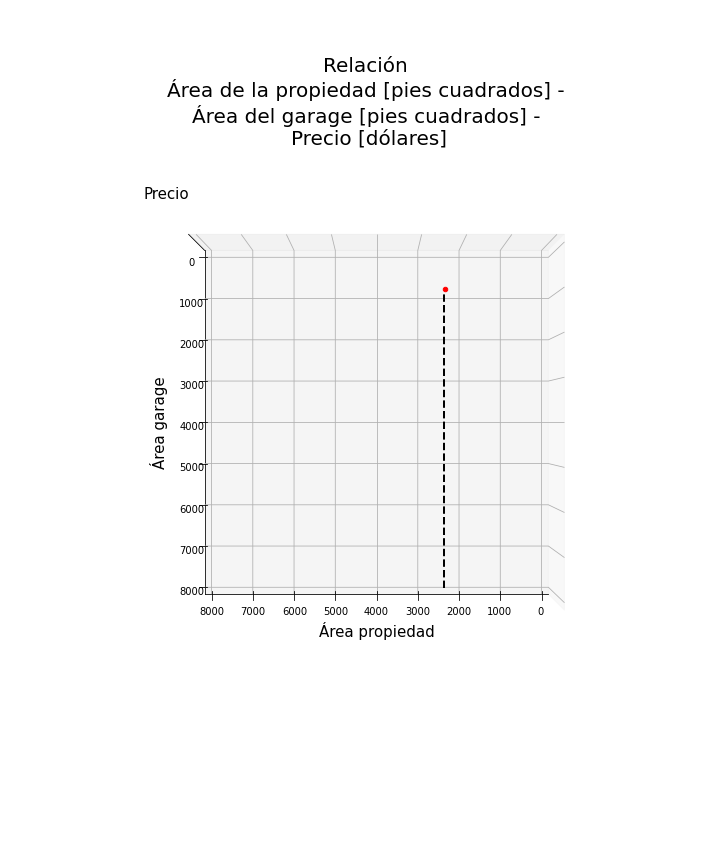
\includegraphics[scale=0.5]{Imagenes/ubicacion_en_x.png}
\centering
\end{figure}
\newpage
\newpage
Luego en el eje y:\\
\begin{figure}[h!]
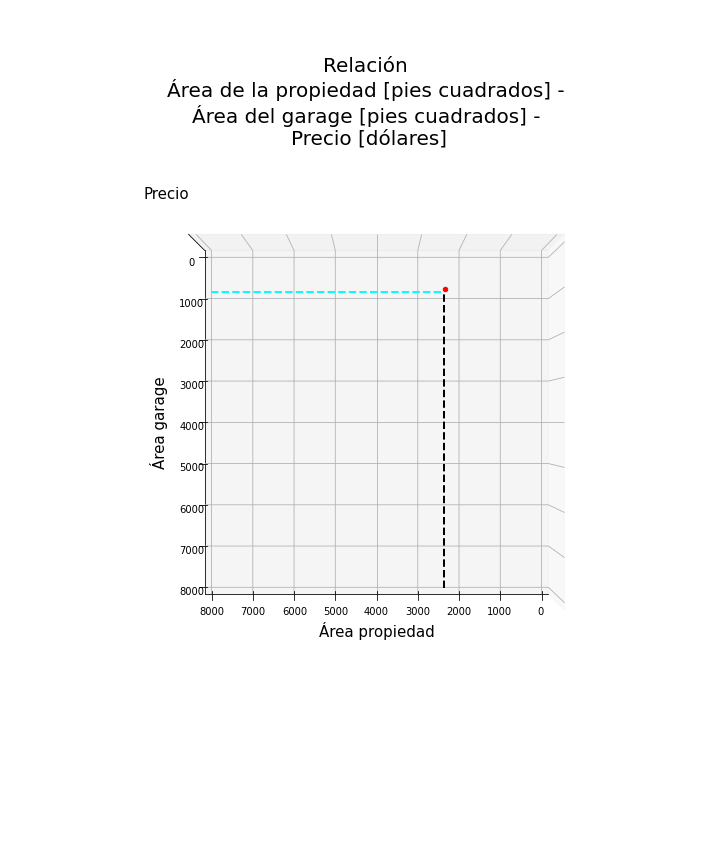
\includegraphics[scale=0.5]{Imagenes/ubicacion_en_y.png}
\centering
\end{figure}
\newpage
Una vez ubicado el punto lo subimos hasta que se ubique en un tercer eje con el precio de la propiedad:\\
% Ubicacion en z
\begin{figure}[h!]
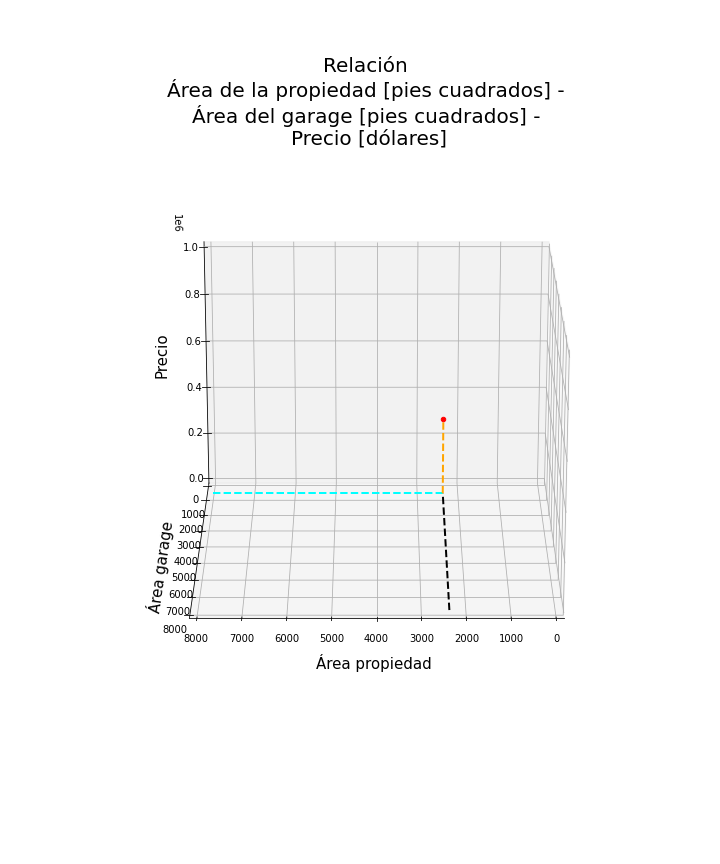
\includegraphics[scale=0.5]{Imagenes/ubicacion_en_z.png}
\centering
\end{figure}
\newpage
Bien, ahora que aprendimos a graficar en 3D grafiquemos el resto de puntos.\\
% Grafico final
\begin{figure}[h!]
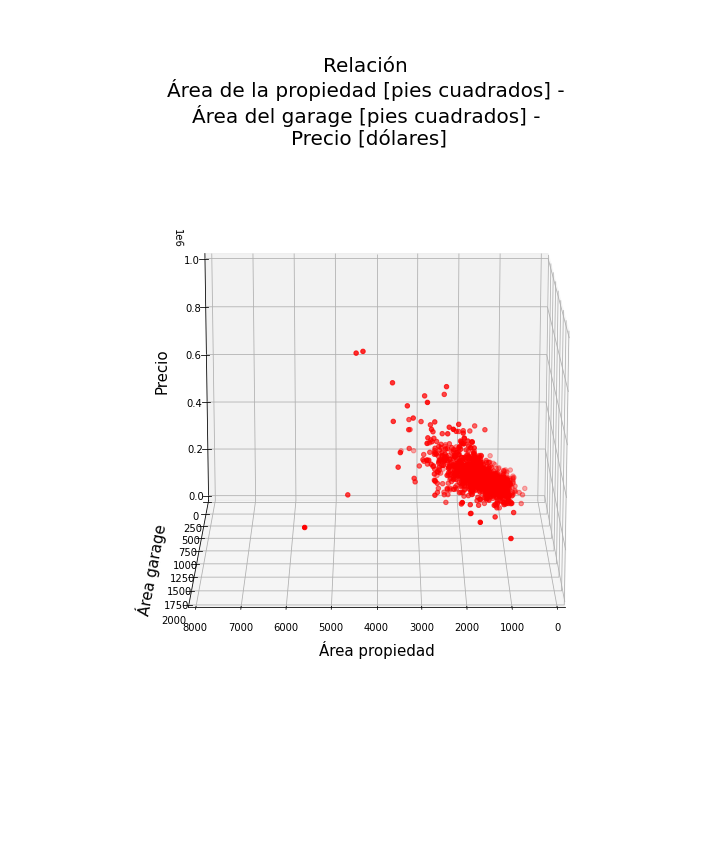
\includegraphics[scale=0.5]{Imagenes/grafico_final.png}
\centering
\end{figure}
\newpage
La pregunta es la misma que antes ¿Como transformamos esa nube indescifrable de puntos en algo que pueda usar? La idea matemática es bastante simple.\\
Ahora vamos a tener 2 variables independientes (x e y) y una variable dependiente (z). La ecuación matemática que modela eso es:
\begin{equation*}
    z=a\cdot x+b\cdot y+c
\end{equation*}
Si somos observadores vemos que se parece a la ecuacion de la recta pero le agregamos el termino $b\cdot y$ . Antes al reemplazar x nos daba valores de y, ahora al reemplazar $(x,y)$ nos da los valores de z.\\
Lo que si cabe aclarar es que el resultado de esto ya no es una recta sino un plano (explicaciones de porque en la parte de fuentes).\\
Este es un ejemplo de como se ve un plano graficado en 3D:\\
% Plano
\begin{figure}[h!]
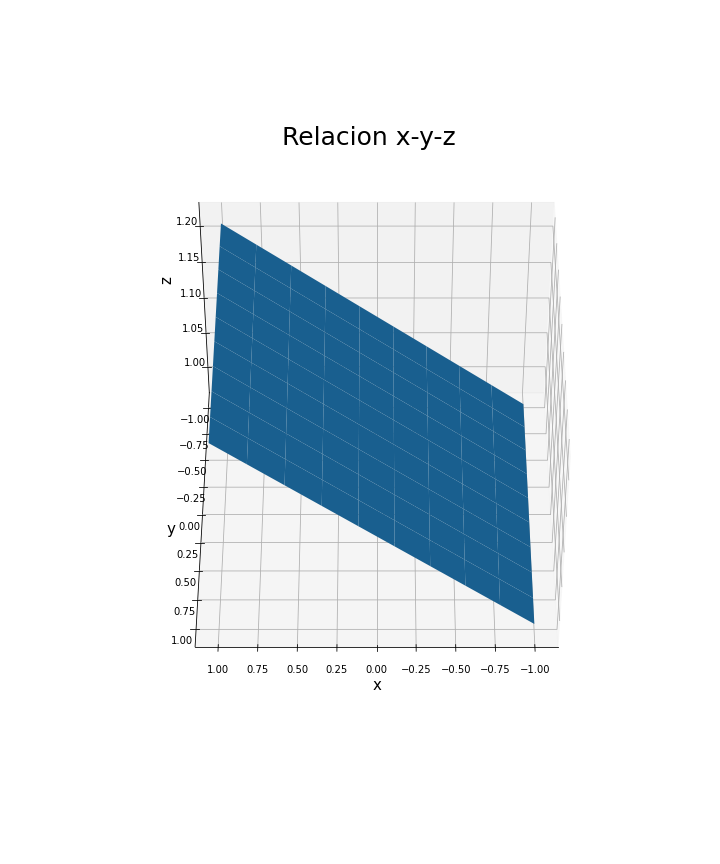
\includegraphics[scale=0.5]{Imagenes/plano.png}
\centering
\end{figure}
\newpage
% Codigo Python
Ahora utilizamos el mismo procedimiento, usamos Python para obtener a, b y c (me ahorro los comentarios del código ya que es muy similar al de la recta).\\
\begin{lstlisting}[language=Python]
import pandas as pd
from sklearn.model_selection import train_test_split
from sklearn.linear_model import LinearRegression

df=pd.read_csv("train.csv")

X = df[['GrLivArea', 'GarageArea']].values.reshape(-1,2)
Y = df['SalePrice']

X_train , X_test , y_train , y_test = train_test_split(X, Y,
    test_size =0.2,random_state=0)

modelo= LinearRegression()
modelo.fit(X_train, y_train)

a=round(modelo.coef_[0],2)
b=round(modelo.coef_[1],2)
c=round(modelo.intercept_,2)
eficiencia_modelo= round(modelo.score(X_test, y_test)*100,2)

print(f"El coeficiente \"a\" del plano es: {a}\n")
print(f"El coeficiente \"b\" del plano es: {b}\n")
print(f"El coeficiente \"c\" del plano es: {c}\n")
print(f"El modelo tiene una eficiencia del {eficiencia_modelo} %")
\end{lstlisting}
Los valores (aproximados a 2 decimales) son estos:\\
\begin{equation*}
    \begin{split}
        a &=81.67\\
        b &=146.23\\
        c &=-12493.3
    \end{split}
\end{equation*}
Y la ecuación del plano es la siguiente:
\begin{equation*}
    z=81.67\cdot x+146.23\cdot y-12493.3
\end{equation*}
Si graficamos este plano tenemos:\\
% Plano aproximacion
\begin{figure}[h!]
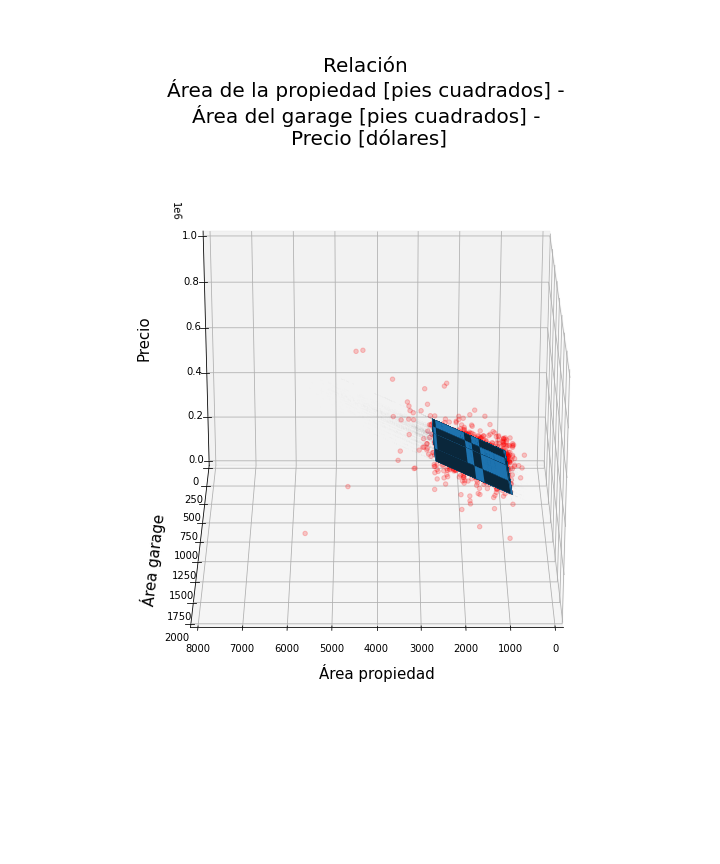
\includegraphics[scale=0.5]{Imagenes/plano_aproximacion.png}
\centering
\end{figure}
\newpage
Y puede tener las mismas aplicaciones que vimos antes con la recta.

\section{¿Como sabemos que estas aproximaciones están bien?}
Una pregunta que nos podemos hacer es ¿Que tan efectivo es mi modelo? ¿Que tanto se equivoca y que tanto acierta?\\
Como vimos en la sección $4$ el modelo dio 43 \% de eficacia ¿Pero que significa este número? ¿Es mucho? ¿Es poco? Siempre es deseable que el porcentaje sea lo mayor posible pero no hay una respuesta única de que numero es el ``correcto” y cual no.\\
Si de 100 casas que tase me equivoque en 57 ¿Me sirve ese modelo para la empresa?\\
Ahora cuando tuvimos en cuenta el área de la propiedad y la cochera ¿Mejoro o empeoro el modelo? Vimos en la sección 7 que la efectividad fue de 51.07 \%. Sin duda un mejor numero, es decir, al aumentar los factores a tener en cuenta mejoro la predicción.\\
Ojo, no porque vaya a tener más factores en cuenta necesariamente que mejore la eficacia del modelo, es más, hasta podría empeorarlo.\\
La idea con lo que hay que quedarse es que es importante medir que tan eficiente es mi modelo, que variables tomo y cual no, cuales tiene sentido, que los modelos son una construcción y que no hay un ``manual” para hacerlo.

\section{Otros modelos de aproximación}
Acá siempre hablamos (en 2 dimensiones) de una recta para aproximar los puntos pero ¿Porque no usar otro tipo de ecuación?\\
Una parábola por ejemplo podría ser otra alternativa para aproximarse al precio de la propiedad. E incluso podríamos pensar otro tipo de funciones (trigonométricas, polinomios, exponenciales, etc).\\
Tranquilos, no se asusten, ya lo iremos viendo en otros textos estas otras ideas.

\section{Último detalle matemático}
Vimos que en 3 dimensiones se puede graficar este problema pero si elegimos 4 dimensiones (área de la propiedad, área de la cochera, año de construcción y precio) se van a complicar las cosas.  Es razonable plantear esto desde un punto de vista analítico (osea, hacer las ecuaciones) pero NO se puede graficar (como hicimos con la recta y el plano). Hay intentos de visualizar más de 3 dimensiones pero son más intentos artísticos que soluciones a problemas matemáticos (al menos de momento).\\
Por eso es importante (entre otras cosas) amigarse un poco con las matemáticas. Porque ayudan a plantear problemas que de otra manera seria imposible.

\section{Fuentes}
\begin{itemize}
    \item \href{https://www.youtube.com/watch?v=k964_uNn3l0}{Video explicando el concepto desde otro punto de vista}
    \item \href{https://scikit-learn.org/stable/modules/generated/sklearn.linear_model.LinearRegression.html}{Documentación de la clase LinearRegression de la libreria sklearn}
    \item \href{https://www.youtube.com/watch?v=3g-e2aiRfbU}{Genial explicación de los conceptos matematicos dentro de la regresión lineal}
    \item \href{https://www.youtube.com/watch?v=3O0DV40B0rs}{Explicación del concepto de 4ta dimension}
    \item \href{https://www.youtube.com/watch?v=MFXKcEeT-M0&list=PLJjOveEiVE4Cbbx1dVjydfmPPpjl0pg86&index=5}{Video explicando el concepto}
    \item \href{https://www.youtube.com/watch?v=YLGhVBB5rGU}{Video aplicando el concepto}
\end{itemize}


\end{document}